\chapter{Декорированная изинговская цепочка}\label{ch:ch3}

При рассмотрении частных случаев обобщенной модели Изинга, мы исследовали единожды декорированную решетку \ref{oneDecorChain}. Рассмотрим данный случай подробнее, а именно, получим точное решение произвольно декорированной цепочки в магнитном поле и исследуем термодинамические, магнитные и фрустрационные свойства декорированной модели Изинга. 

\section{Точное решение декорированной изинговской цепочки в магнитном поле}\label{sec:ch3/sect1}

Запишем гамильтониан произвольно декорированной решетки в следующем виде
\begin{equation}
\mathcal{H}(s) = -J_{d}\sum_{i=1}^{N} s_{i} s_{i+1} - J\sum_{j=1,d+2,\dots}^{N} s_{j}s_{j+d+1} - H \sum_{i=1}^{N} s_{i},
\label{ham}
\end{equation}
где $J_d$ --- обменное взаимодействие между ближайшими декорационными спинами и нодальными спинами, а также между декорационными спинами, $J$ --- обменное взаимодействие только между нодальными спинами, $H$ --- внешнее магнитное поле, $d$ обозначает число так называемых \guillemotleft декораций\guillemotright $ $ цепочки.

 \begin{figure}[h]
 	\center{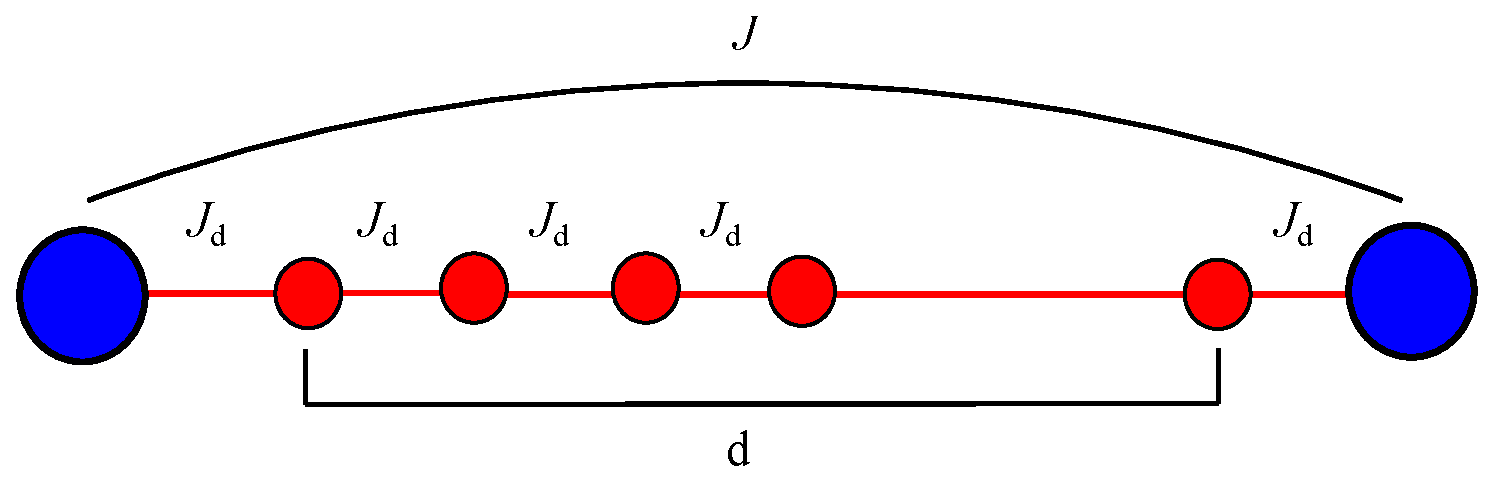
\includegraphics[width=0.7\linewidth]{part3/decorChain.eps}}
 	\caption{Декорированная цепочка с обменным взаимодействием ближайших соседей $J_d$ и обменным взаимодействием $J$}
 	\label{decorChain}
 \end{figure}

На рисунке~\ref{decorChain} изображена решетка спинов, соответствующая декорированной цепочке с гамильтонианом~\eqref{ham}.
Красными кружками обозначены декорационные спины, синими кружками --- основные (нодальные) спины.
Каждый спин обладает двумя состояниями $s=\pm 1$.

Как мы видели, статистическая сумма в термодинамическом пределе ($N\rightarrow \infty$) для единожды декорированной цепочки, то есть при $d=1$, вычисляется из выражения $Z_{N} = \lambda_{\text{max}}^{N/2}$. Статсумма для дважды декорированной цепочки имеет вид $Z_{N} = \lambda_{\text{max}}^{N/3}$, для трижды декорированной цепочки --- $Z_{N} = \lambda_{\text{max}}^{N/4}$ и  т.д. Поэтому легко убедиться в том, что в общем случае выражение для статсуммы с произвольным числом декорирования цепочки примет вид 
\begin{equation}
Z_{N} = \lambda_{\text{max}}^{N/(d+1)}.
\label{zn}
\end{equation}

В формуле \eqref{zn} замечаем, что знаменатель у степени наибольшего собственного значения всегда на единицу больше величины декорирования цепочки $d$. Это означает, что в отсутствие декорационных спинов ($d=0$) цепочка содержит только нодальные спины, таким образом, получаем случай обычной (недекорированной) модели Изинга, статсумма которой вычисляется как $Z_{N} = \lambda_{\text{max}}^{N}$.

Если $d$ устремить к бесконечности, то рассматриваемая задача снова сводится к обычной (недекорированной) модели Изинга, так как при увеличении числа \guillemotleft декораций\guillemotright $ $ относительный вклад в энергию от основных спинов становится все более незначительным.

Согласно алгоритму получения обобщенной трансфер-матрицы Крамерса--Ваннье и применив предложенное Сиози декорационное преобразование (\emph{decoration-iteration transformation})~\cite{siozi_domb1972}, определяем точное выражение для наибольшего собственного значения трансфер-матрицы декорированной цепочки при наличии магнитного поля
\begin{equation}
\lambda_{\text{max}} = \frac{1}{2}\left[e^{\frac{J}{T}}\big(\lambda_1^{d+1} + \lambda_2^{d+1}\big) + e^{-\frac{J}{T}}\big(\lambda_1^{d+1} - \lambda_2^{d+1}\big)\varepsilon \right],
\nonumber
\end{equation}
где 
\begin{align}
\lambda_1 &= \exp{(J_d/T)}[\ch (H/T) + \sqrt{\sh^2 (H/T) + \exp{(-4J_d/T)}}],\nonumber\\
\lambda_2 &= \exp{(J_d/T)}[\ch (H/T) - \sqrt{\sh^2 (H/T) + \exp{(-4J_d/T)}}],\nonumber\\
\varepsilon &= \sqrt{1+\sh^2 (H/T)(\exp(4J/T)-1)/\big(\sh^2 (H/T)+\exp{(-4J_d/T)}\big)}. 	\label{lam}
\end{align}

Термодинамические и магнитные параметры исследуемой декорированной решетки могут быть выражены исключительно через наибольшее собственное значение $\lambda_{\text{max}}$. Тогда, принимая во внимание степень декорирования цепочки $d$, аналитические выражения для энтропии, теплоемкости, намагниченности и параметра порядка, впервые введенного в статье~\cite{kassan-ogly2012}, запишутся следующим образом:
\begin{align}
& S(H,T) = \frac{\ln \lambda_{\text{max}}}{d+1}+\frac{T}{(d+1)\lambda_{\text{max}}}\frac{\partial \lambda_{max}}{\partial T}; \\
& C(H,T) = \frac{T}{(d+1)\lambda_{\text{max}}}\frac{\partial \lambda_{\text{max}}}{\partial T} + \frac{T}{d+1}\frac{\partial }{\partial T}\bigg(\frac{T}{\lambda_{\text{max}}}\frac{\partial \lambda_{\text{max}}}{\partial T}\bigg);\\
& M(H,T) = \frac{T}{(d+1)\lambda_{\text{max}}} \frac{\partial \lambda_{\text{max}}}{\partial H}; \\
& \eta (H,T) = 1-\frac{\ln \lambda_{\text{max}}}{(d+1)\ln 2}-\frac{T}{(d+1)\lambda_{\text{max}} \ln 2}\frac{\partial \lambda_{\text{max}}}{\partial T}.
\end{align} 

\subsection{Термодинамические, магнитные и фрустрационные свойства декорированной изинговской цепочки}

При исследовании модели Изинга на декорированной цепочке в случае антиферромагнитного обмена как между декорационными спинами, так и между основными спинами, в частности, \mbox{$J_d=-1, J=-1$} в магнитном поле $H=2$ при $T\rightarrow 0$, установлено, что энтропию системы (рисунок \ref{entropyDecor}а) можно записать в общем виде для любых значений декорирования $d$
\begin{equation}
\lim_{T \rightarrow 0} S = \frac{1}{d+1} \ln \left[\frac{1}{\sqrt{5}}\left(\varphi^{d+1}-(1-\varphi)^{d+1}\right)\right],
\label{20d}
\end{equation}
где $\varphi=(1+\sqrt{5})/2$ --- золотое сечение.

Таким образом, система в данном режиме фрустрирована, а магнитное поле $H = 2$ является фрустрирующим.

Рисунок \ref{entropyDecor}а демонстрирует, что при стремлении $d$ к бесконечности фрустрирующая энтропия сходится к логарифму золотого сечения. Используя выражение~\eqref{20d}, можно показать, что
\begin{equation}
\lim_{d\rightarrow \infty} \lim_{T \rightarrow 0} S = \lim_{d\rightarrow \infty} \frac{1}{d+1} \ln \left[\frac{1}{\sqrt{5}}\left(\varphi^{d+1}-(1-\varphi)^{d+1}\right)\right] = \ln \varphi.
\label{21d}
\end{equation}

При \mbox{$H=4, J_d=-1, J=-1$} наблюдается еще одно фрустрирующее поле. Фрустрирующая энтропия при разных значениях декорирования (рисунок \ref{entropyDecor}б) представлена в следующем виде
\begin{equation}
\lim_{T \rightarrow 0} S = \frac{1}{d+1} \ln \varphi.
\label{22d}
\end{equation}

 \begin{figure}[h]
 	\begin{minipage}{0.49\linewidth}
 		\center{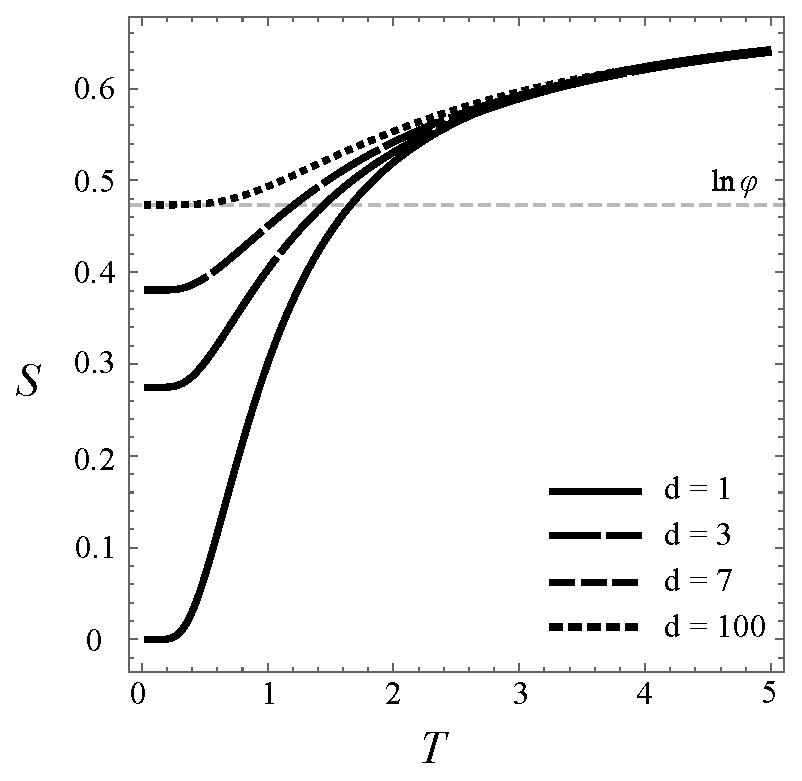
\includegraphics[width=1\linewidth]{part3/entropyDecor1.eps} \\ а)}
 	\end{minipage}
 	\hfill
 	\begin{minipage}{0.49\linewidth}
 		\center{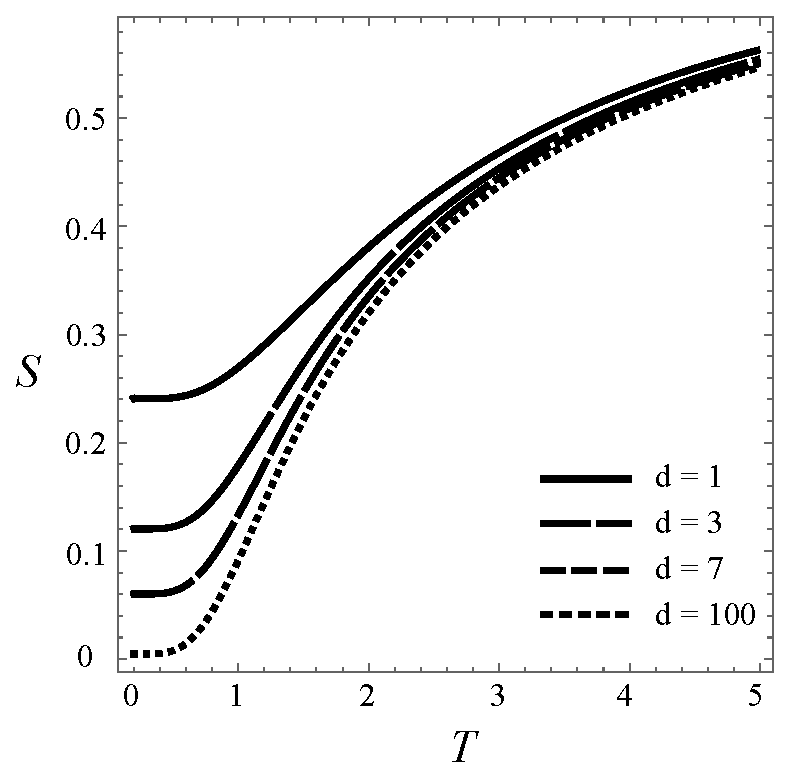
\includegraphics[width=1\linewidth]{part3/entropyDecor2.eps} \\ б)}
 	\end{minipage}
 	\caption{Температурные зависимости энтропий в точках фрустраций антиферромагнитной модели Изинга ($J_d=-1, J=-1$) для различных значений декорирования цепочки: а) в магнитном поле $H=2$;  б) в магнитном поле $H=4$}
 	\label{entropyDecor}
 \end{figure}

Стоит отметить, что при стремлении температуры к бесконечности энтропия равна натуральному логарифму двух 
\begin{equation}
\lim_{T\rightarrow \infty} S = \ln 2,
\label{23d}
\end{equation}
поскольку число состояний на узле равно двум.

Тем не менее, при стремлении температуры к нулю либо к бесконечности теплоемкость при различных параметрах обменных взаимодействий равна нулю (рисунок \ref{heatDecor}а)
\begin{equation}
\lim_{T\rightarrow 0} C = 0,\;\;\;\;\;\;\;\lim_{T\rightarrow \infty} C = 0.
\label{24d}
\end{equation}

Установлено, что в непосредственной близости к точке фрустрации теплоемкость расщепляется на два пика: острый и куполообразный пики. На рисунке \ref{heatDecor}б изображена теплоемкость в точке фрустрации ($H=2$) --- наблюдается единственный куполообразный пик, в то время как в вблизи фрустрации, в частности, в магнитном поле равном $H=1.9$ и $H=2.1$ у теплоемкости появляется дополнительный острый пик. Такое поведение теплоемкости присуще всем фрустрированным системам.

 \begin{figure}[h]
 	\begin{minipage}{0.49\linewidth}
 		\center{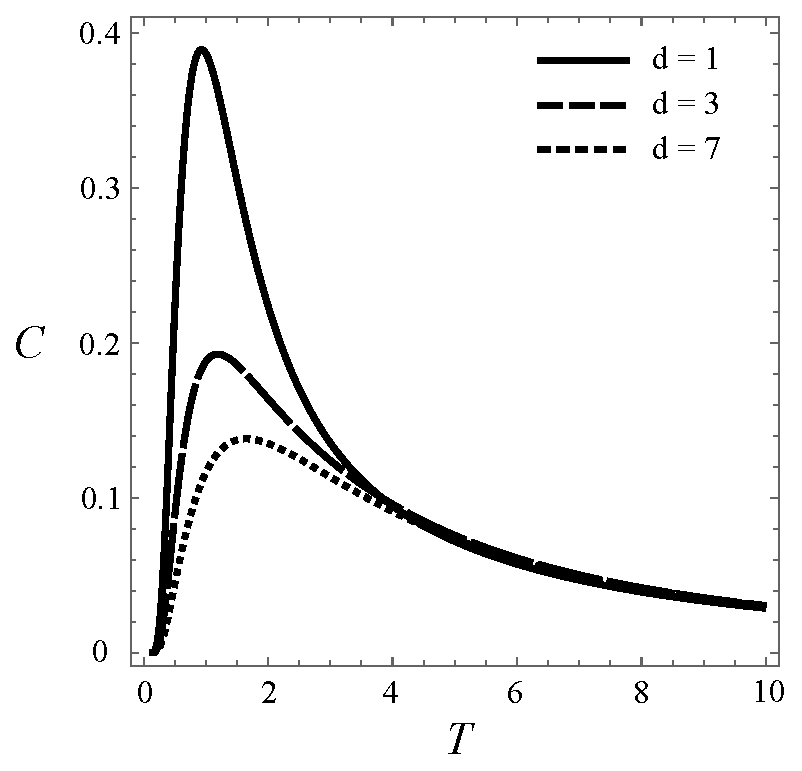
\includegraphics[width=1\linewidth]{part3/heatDecor1.eps} \\ а)}
 	\end{minipage}
 	\hfill
 	\begin{minipage}{0.49\linewidth}
 		\center{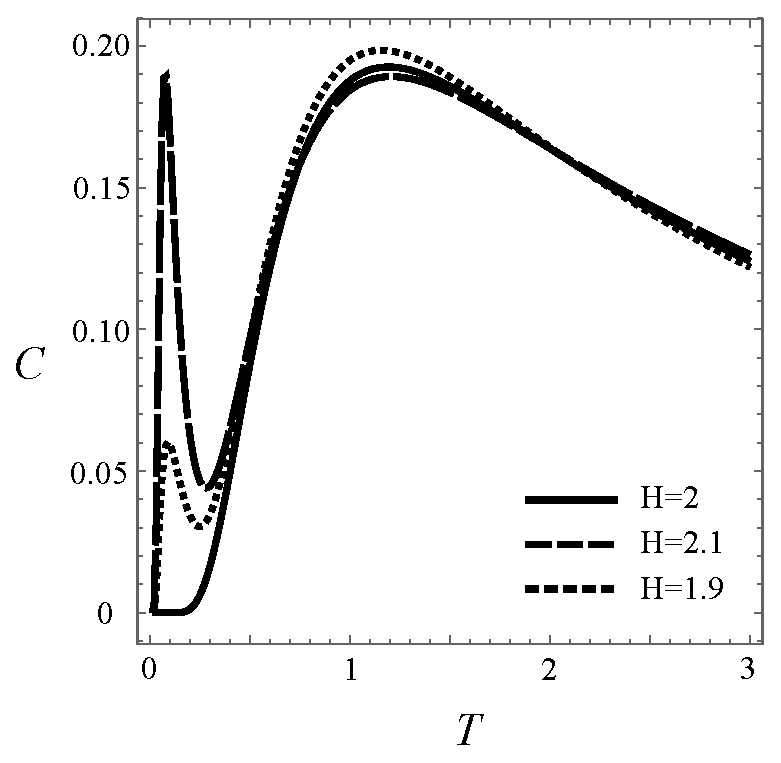
\includegraphics[width=1\linewidth]{part3/heatDecor2.eps} \\ б)}
 	\end{minipage}
 	\caption{Температурные зависимости теплоемкостей при различных значениях декорирования $d$: а) теплоемкость всегда при стремлении температуры к нулю или к бесконечности равна нулю ($H=2$ для всех кривых), б) расщепление теплоемкости на два пика вблизи фрустрации}
 	\label{heatDecor}
 \end{figure}

Намагниченность системы в случае антиферромагнитного обмена спинов решетки при $J_d=-1, J=-1$ во фрустрационном поле $H=2$ и при $T\rightarrow 0$ имеет следующие значения при различных кратностях декорирования $d$ (рисунок \ref{magDecor}а)
\begin{equation}
\lim_{T \rightarrow 0} M = \frac{\Big(d+1-\frac{1}{\sqrt{5}}\Big)\varphi^{d+1}+\Big(d+1+\frac{1}{\sqrt{5}}\Big)(1-\varphi)^{d+1}}{\sqrt{5}(d+1)(\varphi^{d+1}-(1-\varphi)^{d+1})}.
\label{25d}
\end{equation}

Во фрустрационном поле $H=4$ в случае антиферромагнитного обмена спинов решетки \mbox{$J_d=-1, J=-1$} и разных параметрах декорирования получаем следующую фрустрирующую намагниченность (рисунок \ref{magDecor}б)
\begin{equation}
\lim_{T \rightarrow 0} M = \frac{1}{\sqrt{5}}\left(\frac{1+d\sqrt{5}}{d+1}\right).
\label{26d}
\end{equation}

Заметим, что характер поведения намагниченности при антиферромагнитном обменном взаимодействии между спинами при нечетных и четных значениях $d$ различен. При нечетных значениях $d$ намагниченность вблизи фрустрирующего поля, равного двум, разделяется на два промежуточных плато (рисунок \ref{magDecor}а), а при четных $d$ происходит образование исключительно только одного промежуточного плато (рисунок \ref{magDecor}б).

 \begin{figure}[h]
 	\begin{minipage}{0.49\linewidth}
 		\center{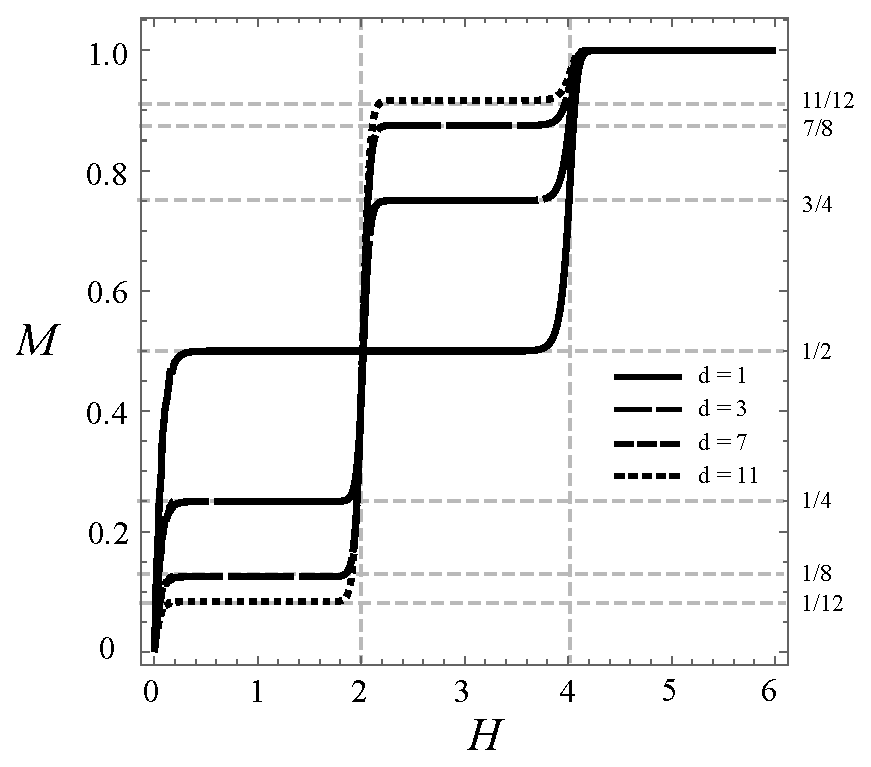
\includegraphics[width=1\linewidth]{part3/magDecor1.eps} \\ а)}
 	\end{minipage}
 	\hfill
 	\begin{minipage}{0.49\linewidth}
 		\center{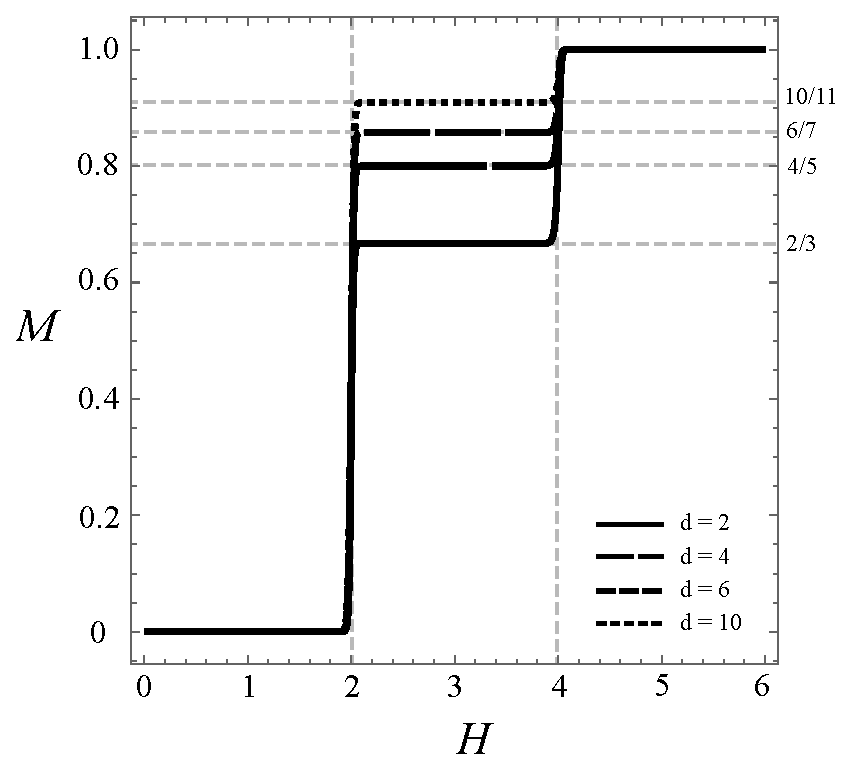
\includegraphics[width=1\linewidth]{part3/magDecor2.eps} \\ б)}
 	\end{minipage}
 	\caption{Намагниченность антиферромагнитной модели Изинга ($J_d=-1, J=-1$) для различных значений декорирования цепочки:  а) нечетные значения $d$ при температуре $T=0.06$;  б) четные значения $d$ при температуре $T=0.02$}
 	\label{magDecor}
 \end{figure}

Рассмотрим взаимодействие спинов иного типа, в частности, обмен между декорационными спинами (и между декорационными и основными спинами) $J_d$ определим антиферромагнитным, а обмен между основными (нодальными) спинами $J$ установим ферромагнитным. Графики температурных зависимостей энтропий в точках фрустраций для разных степеней декорирования продемонстрированы на рисунке~\ref{entropyDecor2}.

 \begin{figure}[h]
 	\begin{minipage}{0.49\linewidth}
 		\center{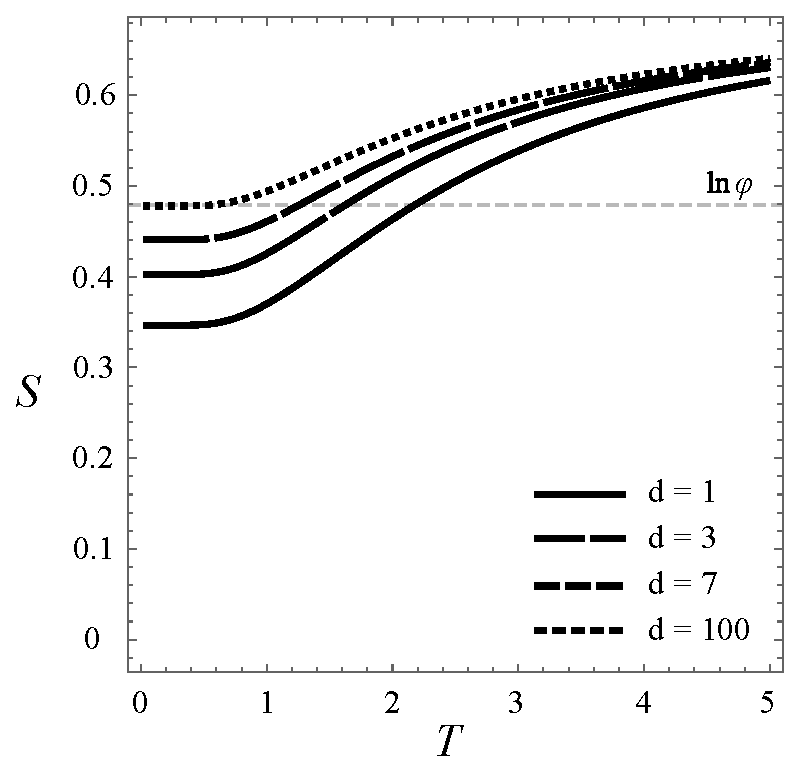
\includegraphics[width=1\linewidth]{part3/entropyDecor3.eps} \\ а)}
 	\end{minipage}
 	\hfill
 	\begin{minipage}{0.49\linewidth}
 		\center{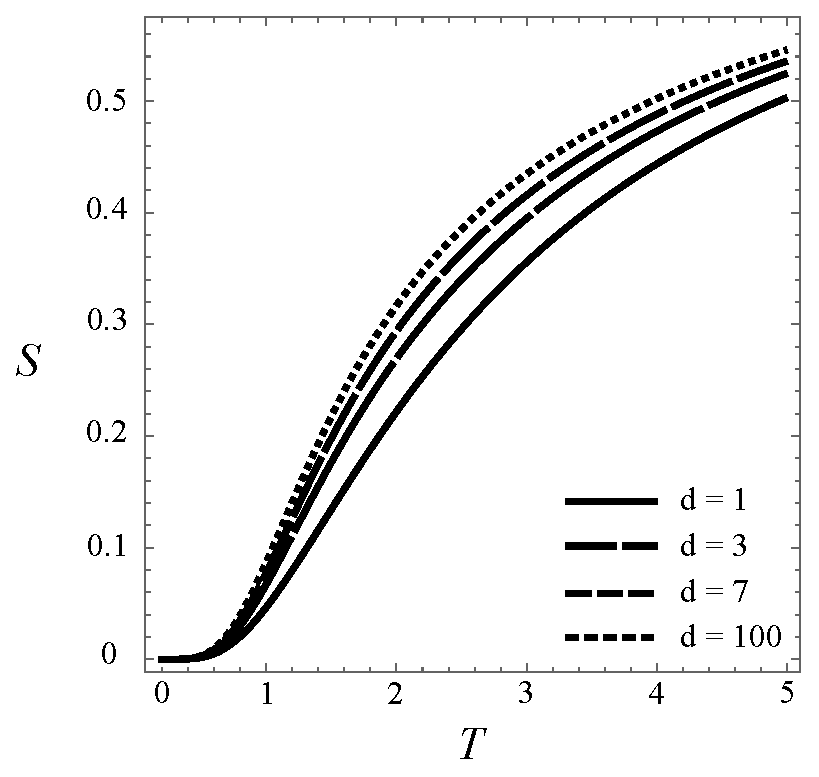
\includegraphics[width=1\linewidth]{part3/entropyDecor4.eps} \\ б)}
 	\end{minipage}
 	\caption{Температурные зависимости энтропий в точках фрустраций антиферро-ферромагнитной модели Изинга ($J_d=-1, J=1$) для различных значений декорирования цепочки: а) в магнитном поле $H=2$;  б) в магнитном поле $H=4$}
 	\label{entropyDecor2}
 \end{figure}

 \begin{figure}[h]
 	\begin{minipage}{0.49\linewidth}
 		\center{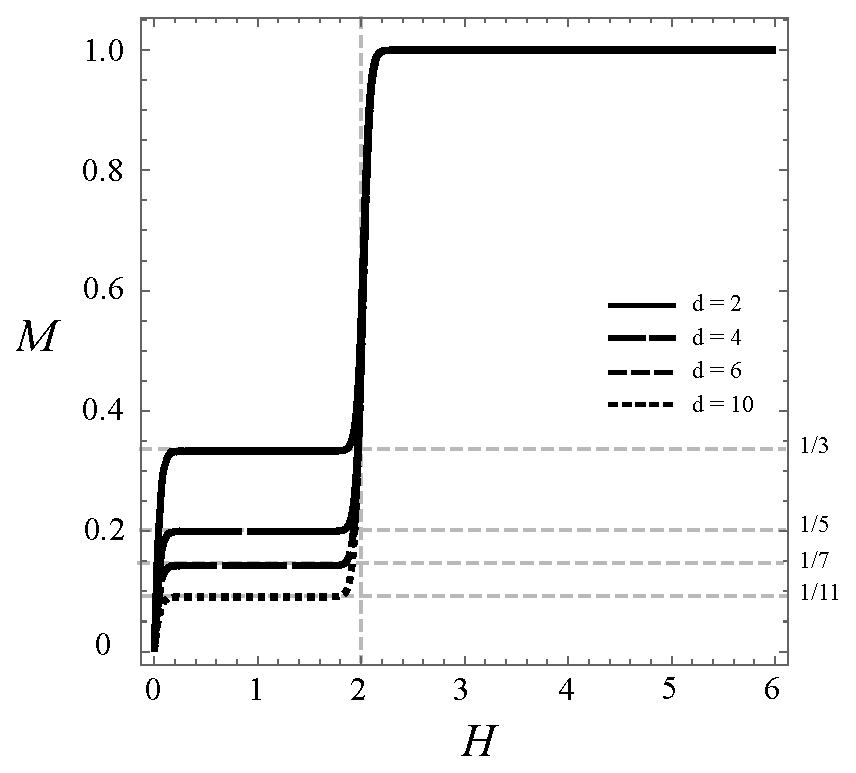
\includegraphics[width=1\linewidth]{part3/magDecor3.eps} \\ а)}
 	\end{minipage}
 	\hfill
 	\begin{minipage}{0.46\linewidth}
 		\center{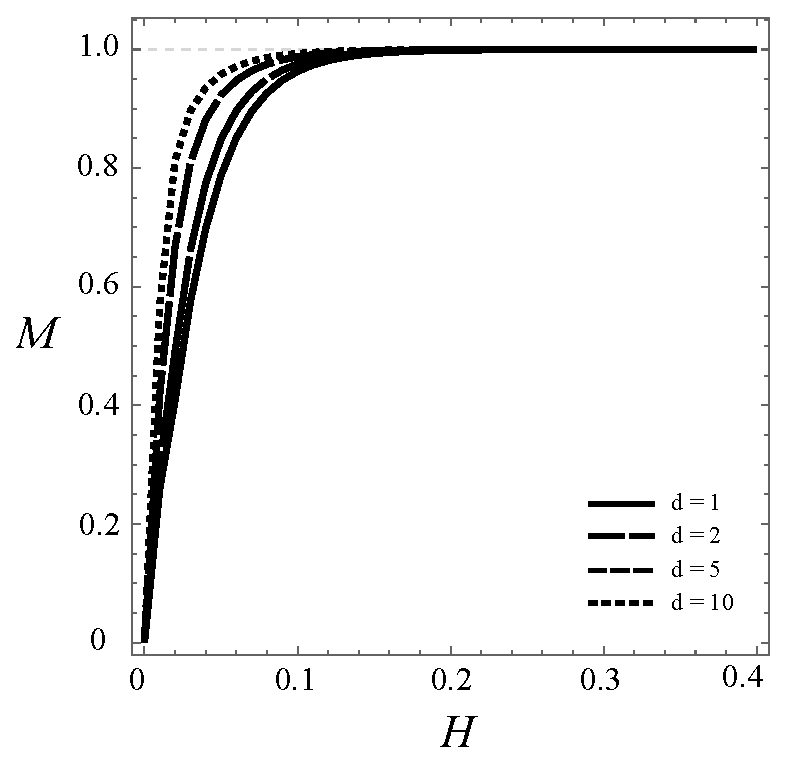
\includegraphics[width=1\linewidth]{part3/magDecor4.eps} \\ б)}
 	\end{minipage}
 	\caption{Намагниченность а) антиферро-ферромагнитной модели Изинга ($J_d=-1$, $J=1$) при температуре $T=0.06$ для четных значений декорирования цепочки;  б) ферро-антиферромагнитной модели Изинга ($J_d=1$, $J=-1$)  при температуре $T=0.06$ для	различных значений декорирования цепочки}
 	\label{magDecor2}
 \end{figure}

При антиферро-ферромагнитном обмене (рисунок \ref{entropyDecor2}а) ($J_d=-1$, $J=1$) во внешнем магнитном поле $H=2$ при $T\rightarrow 0$ фрустрационная энтропия системы выражается следующим образом
\begin{equation}
\lim_{T \rightarrow 0} S = \frac{1}{d+1} \ln \left[\frac{1}{\sqrt{5}}\left(\varphi^{d+2}-(1-\varphi)^{d+2}\right)\right].
\label{27d}
\end{equation}

Соответствующие значения фрустрационных намагниченностей во фрустрационном поле $H=2$ записываются в виде
\begin{equation}
\lim_{T \rightarrow 0} M = \frac{\left(d+2-\frac{1}{\sqrt{5}}\right)\varphi^{d+2}+\left(d+2+\frac{1}{\sqrt{5}}\right)(1-\varphi)^{d+2}}{\sqrt{5}(d+1)(\varphi^{d+2}-(1-\varphi)^{d+2})}.
\label{28d}
\end{equation}

Вместе с тем, во фрустрационном поле $H=4$ замечено, что при различных степенях декорирования решетки, значения фрустрирующих энтропий равны нулю, то есть в этом случае фрустраций не наблюдается, по этой причине, система имеет определенную магнитную конфигурацию в основном состоянии. Этот факт отмечен на рисунке \ref{entropyDecor2}б в случае антиферро-ферромагнитного обмена, помимо этого, на рисунке \ref{magDecor2}а проиллюстрированы намагниченности, описываемые выражениями~\eqref{28d} с фрустрационным полем $H=2$. При четных степенях декорирования $d$ у намагниченности наблюдается только одно промежуточное плато. 

В случае ферро-антиферромагнитного обмена (\mbox{$J_d=1$}, $J\!\!=\!\!-1$), также называемым еще квазиферромагнитным, получаем, что при различных $d$ при сколь угодно малом магнитном поле намагниченность стремится к абсолютному упорядочению вдоль приложенного поля (рисунок \ref{magDecor2}б). 

При ферромагнитном обменном взаимодействии между спинами цепочки ($J_d=1$, $J=1$) при разных значениях параметра $d$ наблюдается подобная ситуация, что и в случае квазиферромагнитного обменного взаимодействия.

Также стоит отметить некоторую особенность поведения намагниченности рассматриваемой декорированной решетки. Установлено, что промежуточные плато намагниченности всегда представляются рациональными дробями. В частности, в случае единожды декорированной цепочки с антиферромагнитным обменом ($J_d=-1$, $J=-1$) имеется промежуточное плато намагниченности со значением $1/2$ (рисунок \ref{magDecor}а), что свидетельствует, что половина спинов развернулось вдоль магнитного поля, в то время как в случае трижды декорированной цепочки плато намагниченностей располагаются на уровнях $1/4$ и $3/4$, и говорят о том, что сначала во фрустрационном поле, равном нулю, повернулась вдоль магнитного поля четверть всех спинов в цепочке, после чего во фрустрационном поле, равном двум, доля повернутых спинов составит три четверти и уже во фрустрационном поле, равном четырем, вдоль магнитного поля развернутся все спины решетки. Несложно определить, что при кратности декорирования, равном $d$, будем иметь плато намагниченности на уровнях $1/(d+1)$ и $d/(d+1)$. А при $d \rightarrow \infty$, замечаем, что промежуточные плато исчезают, а задача сводится к обычной (недекорированной) модели Изинга в магнитном поле с единственным фрустрационным полем равном двум.

 \begin{figure}[h]
 	\center{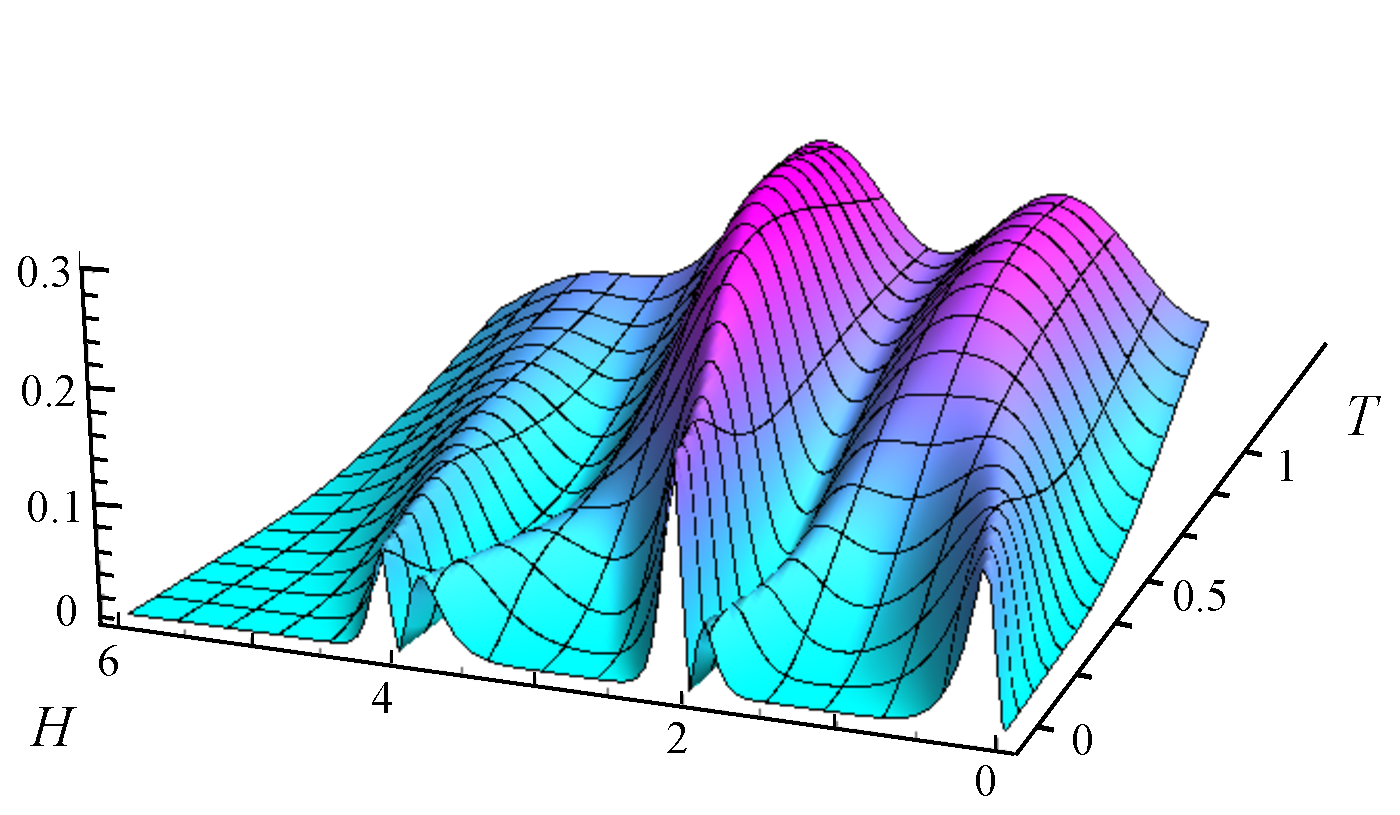
\includegraphics[width=0.77\linewidth]{part3/thirdDecorHeat.eps}}
 	\caption{Теплоемкость трижды декорированной ($d=3$) антиферромагнитной модели Изинга ($J_d=-1, J=-1$) как функция температуры и магнитного поля}
 	\label{thirdDecorHeat}
 \end{figure}

Приступим к описанию термодинамических и магнитных свойств декорированной изинговской цепочки. Для этого построим трехмерные графики теплоемкости и намагниченности как функций температуры и магнитного поля.

Трехмерный график теплоемкости как функции температуры и магнитного поля для трижды декорированной цепочки в случае антиферромагнитного обмена ($J_d=-1$, $J=-1$) изображен на рисунке~\ref{thirdDecorHeat}. Значения магнитного поля, в точках где теплоемкость обращается в нуль (при $T\rightarrow 0$), соответствуют фрустрационным полям. Замечено, что имеется три фрустрационных поля, равные нулю~(cм. статью~\cite{vakbib2}), двум и четырем. В данных фрустрационных полях намагниченность претерпевает скачок, в чем можно убедиться, глядя на рисунок~\ref{thirdDecorMag}.

 \begin{figure}[h]
 	\center{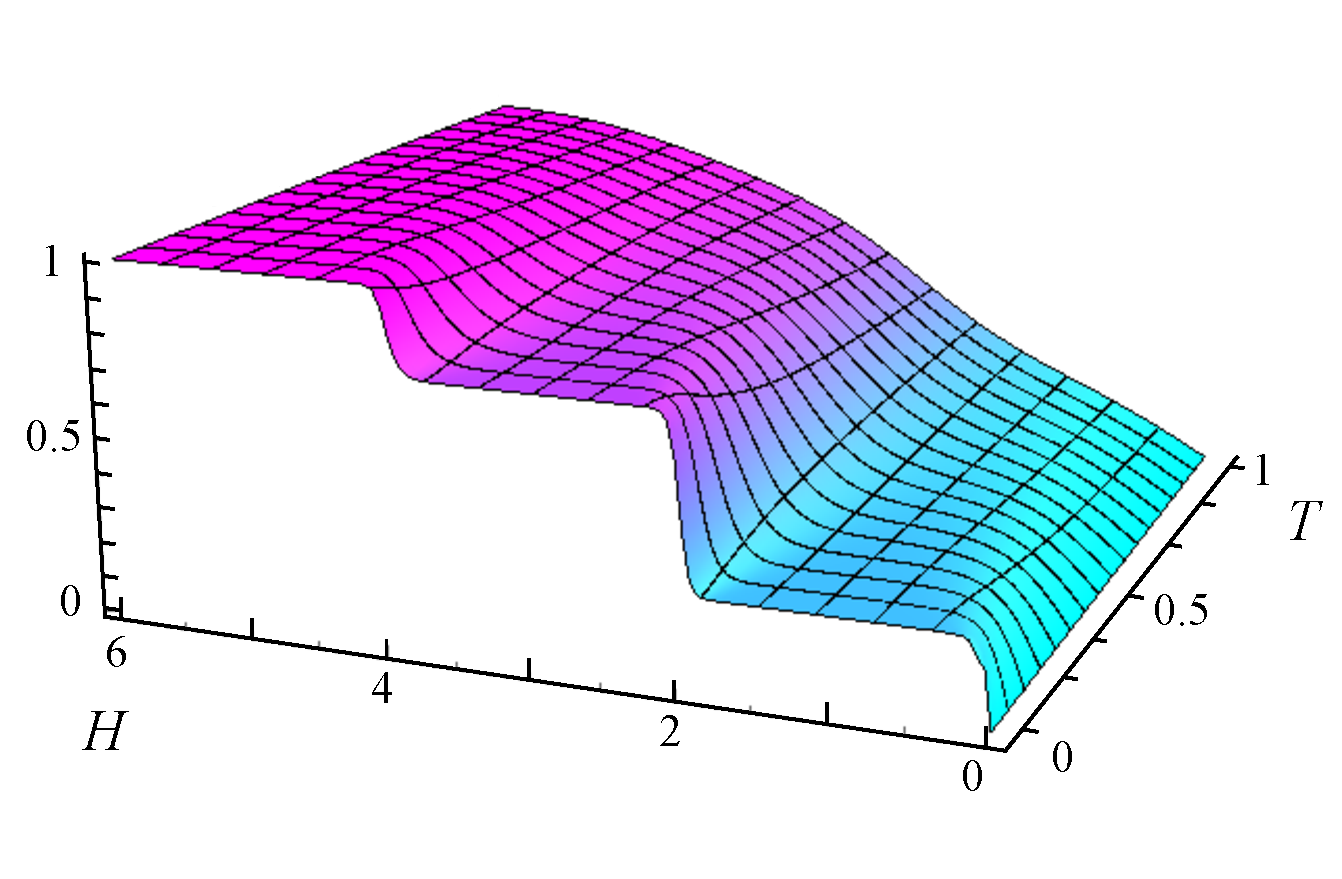
\includegraphics[width=0.77\linewidth]{part3/thirdDecorMag.eps}}
 	\caption{Намагниченность трижды декорированной ($d=3$) антиферромагнитной модели Изинга ($J_d=-1, J=-1$) как функция температуры и магнитного поля}
 	\label{thirdDecorMag}
 \end{figure}

 \begin{figure}[h]
 	\center{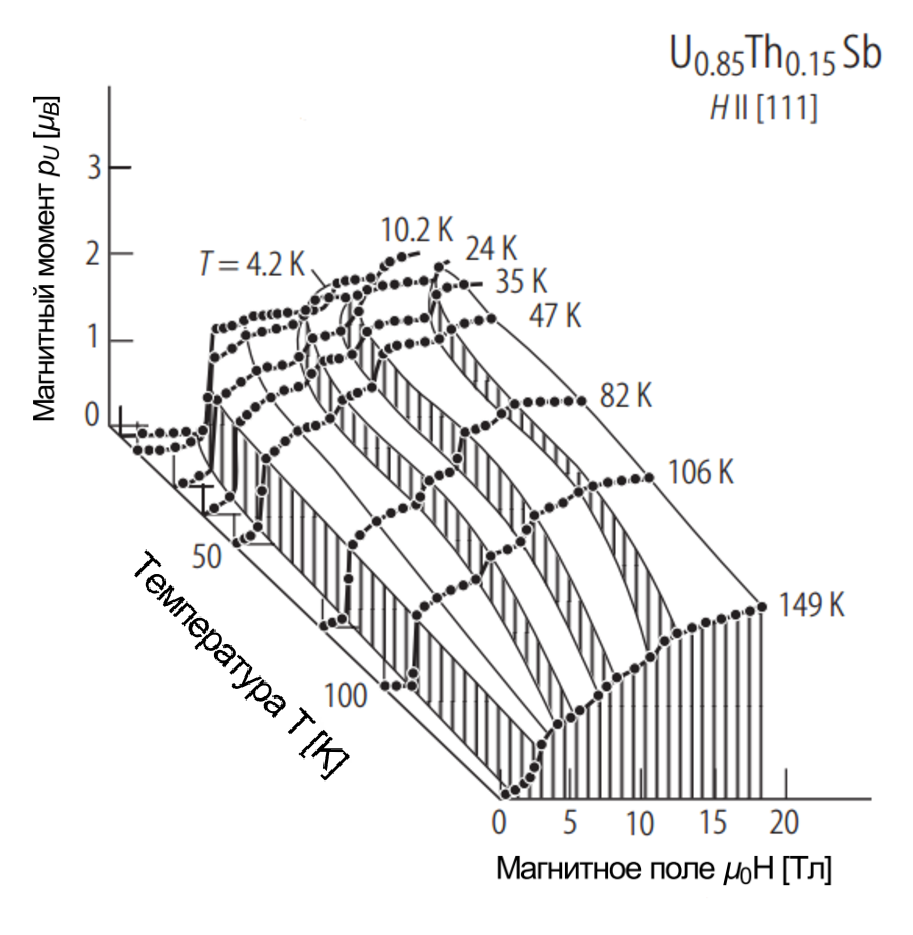
\includegraphics[width=0.7\linewidth]{part3/expMag.eps}}
 	\caption{Экспериментальная намагниченность UThSb~\cite{rossat1982}}
 	\label{expMag}
 \end{figure}

На рисунке~\ref{thirdDecorMag} проиллюстрирован трехмерный график намагниченности как функции температуры и магнитного поля трижды декорированной цепочки в случае антиферромагнитного обмена ($J_d=-1$, $J=-1$). Заметно, что при увеличении температуры кривая намагниченности размывается и промежуточные плато пропадают. 

Можно заметить качественное совпадение между теоретически рассчитанной намагниченностью, изображенной на рисунке~\ref{thirdDecorMag} и полученной экспериментально и проиллюстрированной на рисунке~\ref{expMag}. В обоих случаях имеется ряд скачков намагниченности с низкотемпературными промежуточными плато. При увеличении температуры плато намагниченности также размываются~\cite{rossat1982}. 

 \begin{figure}[h]
 	\begin{minipage}{0.47\linewidth}
 		\center{\includegraphics[width=1\linewidth]{part3/PhaseDiagram1.eps} \\ а)}
 	\end{minipage}
 	\hfill
 	\begin{minipage}{0.47\linewidth}
 		\center{\includegraphics[width=1\linewidth]{part3/PhaseDiagram2.eps} \\ б)}
 	\end{minipage}
 	\caption{Фазовые диаграммы основного состояния системы  декорированной изинговской цепочки в магнитном поле с учетом обменного взаимодействия между ближайшими соседями $J_d=-1$: а) при $d=1$, б) при $d=2$}
 	\label{phaseDiag}
 \end{figure}

Исследуемая декорированная изинговская цепочка зависит от четырех независимых параметров $J_d, J, H, d$, поэтому не представляется возможным изобразить полную фазовую диаграмму, поскольку для этого потребуется четырехмерное пространство. Тем не менее, на рисунке~\ref{phaseDiag} представлены некоторые сечения этого четырехмерного пространства.

Построены магнитные фазовые диаграммы в координатах ($H, J$) для  единожды и дважды декорированной цепочек, находящихся во внешнем магнитном поле (рис.~\ref{phaseDiag}). Замечено, что при $d=1$  в основном состоянии присутствуют три магнитные фазовые конфигурации, а именно, антиферромагнитная фаза $C_2$ с удвоением периода трансляции цепочки 
\begin{equation*}
C_2 =
\left\{\!\begin{aligned}
&\dots \downarrow\;\;\; \uparrow \;\;\;\downarrow \;\;\; \uparrow   \dots\\[1ex]
& \dots \uparrow\;\;\; \downarrow \;\;\;\uparrow \;\;\; \downarrow  \dots
\end{aligned}\right\}
\end{equation*}
с энергией $E_{C_2}^{d=1} = -J/2+J_{d}$, ферромагнитная фаза $C_1$ с сохранением периода трансляции
\begin{equation*}
C_1 =
\left\{\!\begin{aligned}
\dots \uparrow\;\;\; \uparrow \;\;\;\uparrow \;\;\; \uparrow  \dots
\end{aligned}\right\}
\end{equation*}
с энергией $E_{C_1}^{d=1} = -J/2-J_d-H$ и упорядочение $C_4$ с учетверением периода трансляции цепочки 
\begin{equation*}
C_4 =
\left\{\!\begin{aligned}
\dots \uparrow\;\;\; \uparrow \;\;\;\downarrow \;\;\; \uparrow   \dots 
\end{aligned}\right\}
\end{equation*}
с энергией $E_{C_4} = J/2-H/2$ (рисунок~\ref{phaseDiag}a). Все остальные фазы имеют более высокую энергию и оказываются невыгодными в основном состоянии. 

В случае $d=2$ в основном состоянии имеется четыре различных конфигурации: антиферромагнитная $C_2$ с энергией $E_{C_2}^{d=2} = J/3+J_{d}$, ферромагнитная $C_1$ с энергией $E_{C_1}^{d=2} = -J/3-J_d-H$, а также конфигурация $C_3$ c утроением периода трансляции
\begin{equation*}
C_3 =
\left\{\!\begin{aligned}
&\dots \uparrow\;\;\; \uparrow \;\;\;\downarrow   \dots \\[1ex]
&\dots \uparrow\;\;\; \downarrow \;\;\;\uparrow   \dots 
\end{aligned}\right\}
\end{equation*}
с энергией $E_{С_3} = -J/3+J_d/3-H/3$ и фаза $C_6$ с ушестерением периода трансляции
\begin{equation*}
C_6 =
\left\{\!\begin{aligned}
&\dots \uparrow\;\;\; \uparrow \;\;\;\uparrow\;\;\; \downarrow\;\;\; \uparrow \;\;\;\uparrow    \dots \\[1ex]
&\dots \downarrow\;\;\; \uparrow \;\;\;\uparrow\;\;\; \uparrow\;\;\; \uparrow \;\;\;\uparrow    \dots \\[1ex] 
\end{aligned}\right\}
\end{equation*}
с энергией $E_{С_6} = J/3-J_d/3-2H/3$ (рисунок~\ref{phaseDiag}б).

Также, из приведенных диаграмм можно увидеть, что фазы на рисунках сходятся в точке при $J_d=-1, J=0, H=2$. В этой точке схождения фаз нуль-температурная энтропия равняется логарифму золотого сечения, то есть, при таких параметрах задача сводится к обычной (недекорированной) модели Изинга в магнитном поле.

Кроме того, две фазы могут пересекаться на линиях схождения фаз. Такие линии схождения двух фаз, представленные на рисунке~\ref{phaseDiag}, соответствуют определенному обмену --- антиферромагнитному или антиферро-ферромагнитному, которые рассматривались в прошлом разделе. Например, линия схождения фаз $C_1-C_4$ (так же как и $C_1-C_6$) соответствует антиферромагнитному обмену с нуль-температурными энтропиями~\eqref{22} и нуль-температурными намагниченностями~\eqref{26}.

 \begin{figure}[h]
 	\center{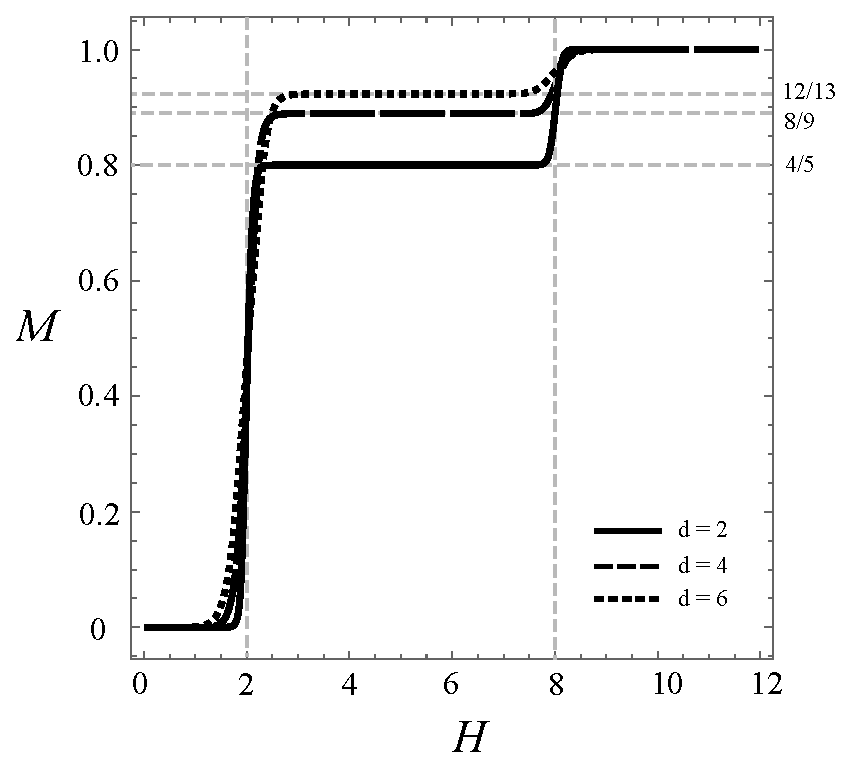
\includegraphics[width=0.55\linewidth]{part3/magDecorSquare.eps}}
 	\caption{Намагниченность антиферромагнитной модели Изинга двукратно-, четырехкратно- и шестикратно-декорированной квадратной решетки ($J_{d_x}=-1, J_{d_y}=-1, J_x=-1, J_y=-1$) при $T=0.005$}
 	\label{magDecorSquare}
 \end{figure}

Вместе с тем, наблюдалось соответствие линейной декорированной цепочки с квадратной декорированной решеткой в магнитном поле~\cite{kassan-ogly2020}. Необходимо подчеркнуть, что расчеты намагниченности в настоящем случае одномерной цепочки следовали из точного аналитического решения~\eqref{14}-\eqref{15}, на квадратной решетке это было возможно выполнить лишь трудоемкими численными расчетами, а именно, методом Монте-Карло в алгоритме Ванга -- Ландау~\cite{wang1,wang2}. В качестве примера на рисунке~\ref{magDecorSquare} приведены намагниченности антиферромагнитной модели Изинга двухкратно-, четырехкратно- и шестикратно-декорированной квадратной решетки. Заметно, что на квадратной декорированной решетке появляются два фрустрационных поля при $H=2$ и $H=8$, в отличие от линейной декорированной цепочки при $H=2$ и $H=4$. Помимо этого, можно обнаружить, что возникшие промежуточные плато намагниченностей как в одномерной (плато расположены на уровнях $1/(d+1)$ и $d/(1+d)$), так и двумерной решетках (плато расположены на уровне $(d_x+d_y)/(1+d_x+d_y)$) при $d \rightarrow \infty$ пропадают, а именно происходит скачок намагниченности из антиферромагнитного состояния прямо в ферромагнитное состояние во фрустрационном поле равном двум, следовательно, задача сводится к обычной (недекорированной) модели Изинга. Объясняется это тем, что с увеличением количества декорационных спинов ($d\rightarrow \infty$) влияние нодальных спинов становится все меньше, в равной степени как на одномерной цепочке, так и на квадратной решетке, что напрямую подтверждается рисунками~\ref{magDecor}, \ref{magDecor2} и~\ref{magDecorSquare}.

\section{Выводы по главе}

Полученные результаты по промежуточным плато намагниченности на декорированных решетках могут быть применены для объяснения многих экспериментальных результатов, где наблюдается качественно схожая картина.

Результаты, описанные в этой главе, опубликованы автором в работах~\cite{confbib3, confbib4, confbib5, vakbib2}.

\FloatBarrier